\documentclass[letterpaper]{article}
\usepackage[utf8]{inputenc}
\usepackage[T1]{fontenc}
\usepackage[spanish]{babel}
\usepackage{amsmath, amsthm, amssymb}
\usepackage{graphicx, float, subcaption, anysize}
\usepackage{listings}
\usepackage{xcolor}

\marginsize{1.5cm}{2cm}{1.5cm}{2cm}

\definecolor{codegreen}{rgb}{0,0.6,0}
\definecolor{codegray}{rgb}{0.5,0.5,0.5}
\definecolor{codepurple}{rgb}{0.58,0,0.82}
\definecolor{backcolour}{rgb}{0.95,0.95,0.92}

\lstdefinestyle{mystyle}{
    backgroundcolor=\color{backcolour},   
    commentstyle=\color{codegreen},
    keywordstyle=\color{magenta},
    numberstyle=\tiny\color{codegray},
    stringstyle=\color{codepurple},
    basicstyle=\ttfamily\footnotesize,
    breakatwhitespace=false,         
    breaklines=true,                 
    captionpos=b,                    
    keepspaces=true,                 
    numbers=left,                    
    numbersep=5pt,                  
    showspaces=false,                
    showstringspaces=false,
    showtabs=false,                  
    tabsize=2
}

\lstset{style=mystyle}
\setlength{\parindent}{0cm}
\begin{document}

%\renewcommand{\refname}{Bibliografía}
\begin{figure}
    \subfloat{
\includegraphics[width = 0.2\textwidth]{img/unamescudo}}
    \hfill
    \subfloat{
\includegraphics[width = 0.2\textwidth]{img/escudofi_negro}}
\end{figure}

\begin{titlepage}
    \centering
    {\bfseries\LARGE UNIVERSIDAD NACIONAL AUTÓNOMA DE MÉXICO \par}
    \vspace{1cm}
    {\bfseries\LARGE FACULTAD DE INGENERÍA \par}
    \vspace{1cm}
    {\bfseries\LARGE DIVISIÓN DE INGENIERÍA ELÉCTRICA \par}
    \vspace{1cm}
    {\itshape\Large\textbf{Asignatura: Compiladores (0434)}\par}
    \vspace{1cm}
    {\itshape\Large\textbf{Proyecto: Analizador Sintáctico Ascendente}\par}
    \vspace{1cm}
    {\itshape\Large \textbf{Profesor: Ing. Manuel Castañeda Castañeda}\par}
    \vspace{1cm}
    \vfill
    {\itshape\Large \textbf{Integrantes del equipo:}\\\par}
    \begin{itemize}
        \centering
        {\itshape\Large
        \item [\textbullet] Bautista Pérez Brian Jassiel
        \item [\textbullet] González Ramírez David
        \item [\textbullet] Guillén Castro Jorge Luis
        \item [\textbullet] Meneses Gómez Iassiel Navih}
    \end{itemize}
    \vfill
    {\itshape\Large Grupo: 05\par}
    {\itshape\Large \textbf{Semestre: 2022-2}\par}
    {\itshape\Large \textbf{Fecha de entrega: \today}\par}
\end{titlepage}

\tableofcontents

\newpage

\section{Introducción}
El compilador es una herramienta que permite el traducir un lenguaje de programación a otro
para su futura interpretación, el cuál maneja un análisis del código origen, para efectos de este
proyecto se hizo enfásis en el análizador sintáctico.

El analizador sintáctico, también conocido como parser, representa la segunda
fase de compilación, se encarga de realizar un análisis mediante las
gramáticas para verificar si la sintaxis de la instrucción es adecuada para el programa, una
vez realizado esto se genera un árbol sintáctico, el cual puede ser ascendente o descendente. 

Para este proyecto, se implementó un árbol sintáctico ascendente, la construcción se
realiza desde las hojas más externas del árbol y van poco a poco subiendo a sus raíces, esto
se puede entender como una entrada, la cual va generando pequeñas derivaciones hasta
llegar al axioma inicial.

Para la correcta realización del proyecto se va a implementar un analizador sintáctico
ascendente de acuerdo a una gramática dada, donde el analizador léxico tendra que reconocer
los números reales, identificadores, operadores y paréntesis, por lo cual se podrá indicar
si la cadena es válida o no.


\section{Desarrollo}
Se debe de elaborar un analizador sintáctico ascendente que revise las sentencias
de acuerdo a la siguiente gramática:
$E \rightarrow T$ \\
$E \rightarrow E + T$ \\
$E \rightarrow E - T$ \\
$T \rightarrow i$ \\
$E \rightarrow (E)$ \\
i - Será cualquier número real o identificador.

Se utilizó el lenguaje Java para la implementación del código de nuestro analizador sintáctico.

\textbf{Analizador sintáctico ascendente}

A lo largo del curso se vio que un analizador léxico es aquel que conforma la primera fase
de la compilación  y está destinado a leer caracteres del archivo de entrada, donde se
encuentra la cadena a analizar, reconocer subcadenas que correspondan a símbolos del lenguaje
y retomar los tokens correspondientes y sus atributos. Además procesa los lexemas que le va a 
suministrar el analizador sintáctico y verificará que estén bien ordenados, si no lo están
se generarán errores.

A continuación, el código:

\lstinputlisting[language=Java]{bottomUpParser.java}

\section{Análisis de resultados}
A continuación el árbol sintáctico hecho de manera manual junto con su análisis:

\textbf{Gramática.}

$1) E \rightarrow T$ \\
$2) E \rightarrow E + T$ \\
$3) E \rightarrow E - T$ \\
$4) T \rightarrow i$ \\
$5) E \rightarrow (E)$ \\

\textbf{Cadena de Entrada.}
$i-(i+3.4)$

$4) T \rightarrow i - (i + T)$ \\
$4) T \rightarrow i - (T + T)$ \\
$1) E \rightarrow i - (E + T)$ \\
$2) E \rightarrow i - (E)$ \\
$5) T \rightarrow i - i + T$ \\
$4) T \rightarrow T - T $ \\
$1) E \rightarrow E - T$ \\
$3) E \rightarrow E$ \\

\textbf{Cadena transformada con la gramática para realizar el analizador sintáctico ascendente:}
$i-(i +i)$

$3) E \rightarrow E - T$ \\
$1) E \rightarrow T - T$ \\
$4) T \rightarrow i - T$ \\
$5) T \rightarrow i - (E)$ \\
$2) E \rightarrow i - (E + T)$ \\
$1) E \rightarrow i - (T + T)$ \\
$4) T \rightarrow i - (i + T)$ \\
$4) T \rightarrow i - (i + i)$ \\

\begin{figure}[H]
    \centering
    \begin{subfigure}{0.45\textwidth}
        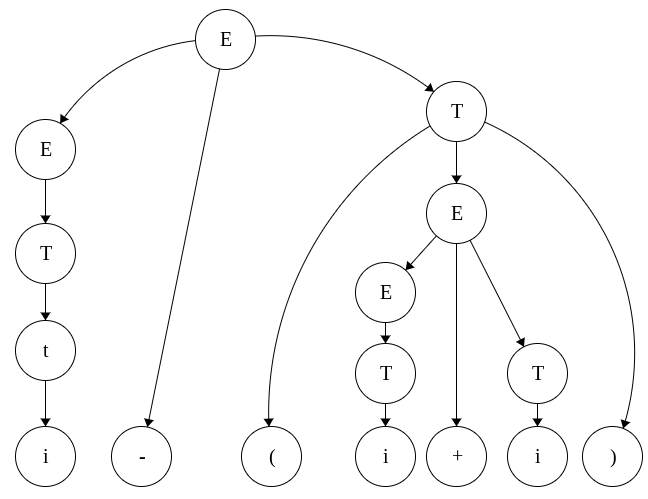
\includegraphics[width=\textwidth]{img/arbol_sint}
        \caption*{Árbol Sintáctico Ascendente.}
    \end{subfigure}
\end{figure}

\section{Conclusiones}
Aquí van las Conclusiones
\end{document}